\chapter{IMPORTANCE OF SEDIMENT GRAIN SIZE TO STOCKS AND STABILITY OF ORGANIC CARBON BURIED IN SEAGRASS SOILS}		\label{another chapter}

\section{Abstract}
Seagrass ecosystems are being considered for conservation and management projects aimed at climate change mitigation based on the organic carbon (C\textsubscript{org}) that they have historically sequest....

\section{Introduction}


The capability of some coastal ecosystems to sequester CO\textsubscript{2} and store large carbon stocks is drawing increasing attention as a means of inexpensive, conservation-based climate change mitigation \citep{Hiraishi:2014uo}. The term “Blue Carbon” is used to describe the vulnerable organic carbon stocks associated with these coastal vegetated ecosystems (seagrass meadows, mangrove forests, and tidal marshes) that could be lost and emitted as CO\textsubscript{2} during habitat destruction or degradation \citep{Mcleod:2011gs}. The term is also tied to those carbon finance policies and frameworks under development to maximize carbon sequestration through the protection and promotion of carbon-rich ecosystems (collectively called “Blue Carbon strategies”; \citealt{Pendleton:2012hz}). Pressure to quantify Blue Carbon stocks and assess the relative risk of CO\textsubscript{2} emissions from degraded sites is spurring a flood of investigations into the causal connections between manageable ecosystem attributes and stable, long-term carbon sequestration \citep{Howard:2017jz, Macreadie:2017dt}. Discussio....

\bigskip
\noindent Drivers of C\textsubscript{org} stocks in Seagrass Ecosystems
\medskip

Soil C\textsubscript{org} stocks associated with seagrass ecosystems vary greatly among sites, influenced by local seagrass-related features, but also local geomorphological and hydrological setting as well as soil characteristics \citep{Serrano:2016cv}. When considered broadly, seagrass ecosystems promote C\textsubscript{org} storage, with studies showing that seagrass presence \citep{Macreadie:2015hc, Mazarrasa:2015gv}, density and productivity \citep{Serrano:2014ho}, and recolonization \citep{Greiner:2013wi, Marba:2015hj} are all positively correlated with soil carbon storage. Seagrasses directly contr......

\bigskip
\noindent Decomposition and CO\textsubscript{2} Production in Seagrass Ecosystems
\medskip

Mapping dense seagrass organic carbon stocks has taken primacy in Blue Carbon efforts, though for stocks to be relevant in discussions of greenhouse gas emissions, there must be evidence that seagrass-mediated attributes are linked to changes in organic matter remineralization, and hence, CO\textsubscript{2} production rates. In other words, for seagrasses to be important in controlling seagrass soil C\textsubscript{org} stocks, seagrass presence must prevent decomposition and remineralization that would otherwise occur in their absence. In seagrasses, like other Blue Carbon ecosystems, the production of CO\textsubscript{2} is driven mainly by respiratory processes linked to the decomposition and remineralization of organic matter (OM). The stability and permanence of C\textsubscript{org}) stocks is typically attributed to suppressed microbial activity and resultant low breakdown rates when buried in the relatively stable, low redox, anoxic soils \citep{Duarte:2011da, Fourqurean:2012cv}. The loss of ....

\section{Materials and Methods}


The Florida Keys National Marine Sanctuary and Florida Bay cover over 11000 km\textsuperscript{2} and host the largest documented continuous seagrass ecosystem in the world \citep{Fourqurean:2002wr}. Seagrass communities across the south Florida seascape are composed primarily of \textit{Thalassia testudinum}, \textit{Halodule wrightii}, and/or \textit{Syringodium filiforme} depending on local nutrient availability, sediment type, salinity, and light availability, among other factors \citep{Fourqurean:1995uj, Fourqurean:2003vj}. During the summer and winter seasons of 2015 and 2016, 45 sites were surveyed for depth, sediment type, average canopy height, and species-specific seagrass abundance, as part of ongoing seagrass monitoring programs that have been underway for over 20 years \citep{Fourqurean:2002wr}. A map of the region with study can be found in (Figure~\ref{fig:2F0}). ....

\bigskip
\noindent Data Processing
\medskip

The Braun–Blanquet scale is an effective method for the rapid assessment of benthic coverage, though the 0 - 5 scale is both non-linear and categorical, greatly limiting statistical usefulness. Species-specific Braun-Blanquet scores were converted to percent coverage by assigning the median percent cover of each score’s coverage range for each quadrat along the transect. Thus, a score of 5, representing 75 \% - 100 \% coverage, is converted to 87.5 \% coverage (Table~\ref{table:2T1}). The calculated species-specific percent coverages at each quadrat were added together for total seagrass coverage. Species-specific and total seagrass coverage percentages were averaged across all quadrats from each site’s 50 m transect (n = 10), then site-specific coverage density averages (in \% cover) were averaged again across sampling campaigns over two years (n = 4) to account for both minor spatial and temporal variations in a site’s seagrass coverage. Similar procedures were applied to categorical sediment type data; sediment categories were assigned numbers one through nine of increasing coarseness, where “1” is mud and “9” is rock (Table~\ref{table:2T2}) These scores were averaged across a site’s transect, then across sampling campaigns for a representational sediment score. Numerical scores were back-calculated to original categorical nomenclature for easy interpretation. Average canopy height for each site was calculated by averaging measurements across each site’s transect, then averaging across sampling campaigns.

\bigskip
\noindent Data Analysis
\medskip

When making pairwise comparisons of continuous variables (seagrass coverage, C\textsubscript{org} cont....


\section{Results}


\bigskip
\noindent Soil C\textsubscript{org}
\medskip

Soil C\textsubscript{org} content ranged from 0.7 \% to 8.6 \% averaging ....

\bigskip
\noindent Seagrass Characteristics
\medskip

Seagrass was present at 96 \% of sites during sampling period. \textit{Thalassia testudinum} was the most ....

\bigskip
\noindent Sediment Grain Size
\medskip

Sediment type varied greatly across the South Florida seascape with sites within the protected water of Florida Bay and the Gulf of Mexico side of the lower Florida Keys containing sediments categorized exclusively as mud or sandy mud (Figure~\ref{fig:2F3}b). Other sites showed a greater variation in sediment type, with deeper oceanside sites generally having coarser (muddy sand, sand, or gravel) sediments. Categorical sediment classifications collected through long-term monitoring correlated with traditionally measured sediment type indicators; sites with lower sediment index scores (i.e., mud and sandy mud) had higher fractions of mud (Figure~\ref{fig:2F5}a; ANOVA, p < 0.05) and generally lower dry bulk densities (Figure~\ref{fig:2F5}b; ANOVA, p < 0.05) ....


\section{Discussion}

Successful Blue Carbon management in seagrass ecosystems relies on the protection of large seagrass C\textsubscript{org} stocks where OM remineralization rates are low. Here we show that seagrass density and canopy height are related to surface C\textsubscript{org} stocks across the South Florida seascape, though sediment type and grain size (not necessarily driven by seagrasses) better explain variation in C\textsubscript{org} soil stocks. Sediment characteristics, rather than seagrass characteristics, controlled OM breakdown rates. Rates of OM degradation were only slower for buried compared to surficial sediments at sites with fine-grained, high C\textsubscript{org} soils. Conversely, rates of OM breakdown were higher when buried in coarse-grained, low C\textsubscript{org} seagrass sediments than they were at the sediment surface. These finding have direct bearing on the development of Blue Carbon strategies, as they suggest that only sites with fine sediments enhance perservation of C\textsubscript{org} through burial, regardless of seagrass presence.

The sediment C\textsubscript{org} content across South Florida (averaging 2.4 $\pm$ 0.3 \% ) was ....

\bigskip
\noindent Implications for Management and Blue Carbon Strategies
\medskip

Best practices for Blue Carbon management involve assessments of the C\textsubscript{org} that could be remineralized and lost as greenhouse gases \citep{Howard:2017kp}. These risk assessments can include a loss of C inputs, but more importantly, the size of C\textsubscript{org} stocks that could be lost as well as the potential that stocks are susceptible to enhanced remineralization if disturbed \citep{Lovelock:2017ez}. Studies to date focus on quantifying stocks, making site and regional assessments of C\textsubscript{org} storage, and understanding ecological and environmental correlates. For C\textsubscript{org} stocks to be important to climate mitigation and Blue Carbon management, we need to also understand whether C\textsubscript{org} stocks can be remineralized, the environmental conditions that control remineralization, and best management practices that could keep C\textsubscript{org} sequestered.
......



\section{Acknowledgements}

Christian Lopes, Claudia Carrión, Sara Wilson, and James Fourqurean are coauthors of the independent, manuscript version of this chapter. David Barahona, Kai Lopez, and Alex Perez helped collect, prepare and process samples for nutrient analysis. This research was conducted through the Florida Keys National Marine Sanctuary seagrass monitoring program funded by the US Environmental Protection Agency under Contract No. X7 95469210, and the Florida Coastal Everglades Long-Term Ecological Research program under National Science Foundation Grant DEB-1237517. Further support was provided by a Dissertation Year Fellowship from FIU.

\section{\normalfont{Work Cited}}
\begingroup
\setlength{\bibsep}{10pt}
\linespread{1}\selectfont


\renewcommand{\section}[2]{}%
\bibliographystyle{apalike}
\bibliography{wholebib2}
\endgroup
\newpage

\begin{figure}[t]
  \centering
   \includegraphics[width=.99\textwidth,clip, trim={1.5cm 3.5cm 0.5cm 1.9cm}]{Figures/chapter2/F0}
\caption[Regional map including sites]{Map of South Map including study sites and sites where canvas strips were successfully recovered}
  \label{fig:2F0}
\end{figure}

\begin{table}[t]
  \centering
  \includegraphics[width=.99\textwidth,clip, trim={1.7cm 12.6cm 5.2cm 2.5cm}]{Figures/chapter2/T1}
\caption[Description of modified Braun-Blanquet abundance scores]{Modified Braun-Blanquet abundance scores, their description, and their assigned percent coverage}
  \label{table:2T1}
\end{table}


\begin{table}[t]
  \centering
  \includegraphics[width=.99\textwidth,clip, trim={1.7cm 2.5cm 6.5cm 3.2cm}]{Figures/chapter2/T2}
\caption[Sediment categories and their assigned ranking of increasing coarseness]{Sediment categories and their assigned ranking of increasing coarseness}
  \label{table:2T2}
\end{table}


\begin{figure}[t]
  \centering
   \includegraphics[width=.99\textwidth,clip, trim={1.7cm 2.5cm 1.0cm 3.2cm}]{Figures/chapter2/F1}
\caption[Canvas assay deployment apparatus]{Depiction of single canvas assay deployment apparatus. Strips were deployed at each site (n=10) at the sediment-water interface and 20 cm depth with foam buoy for easy detection and recovery.}
  \label{fig:2F1}
\end{figure}

\begin{table}[t]
  \centering
  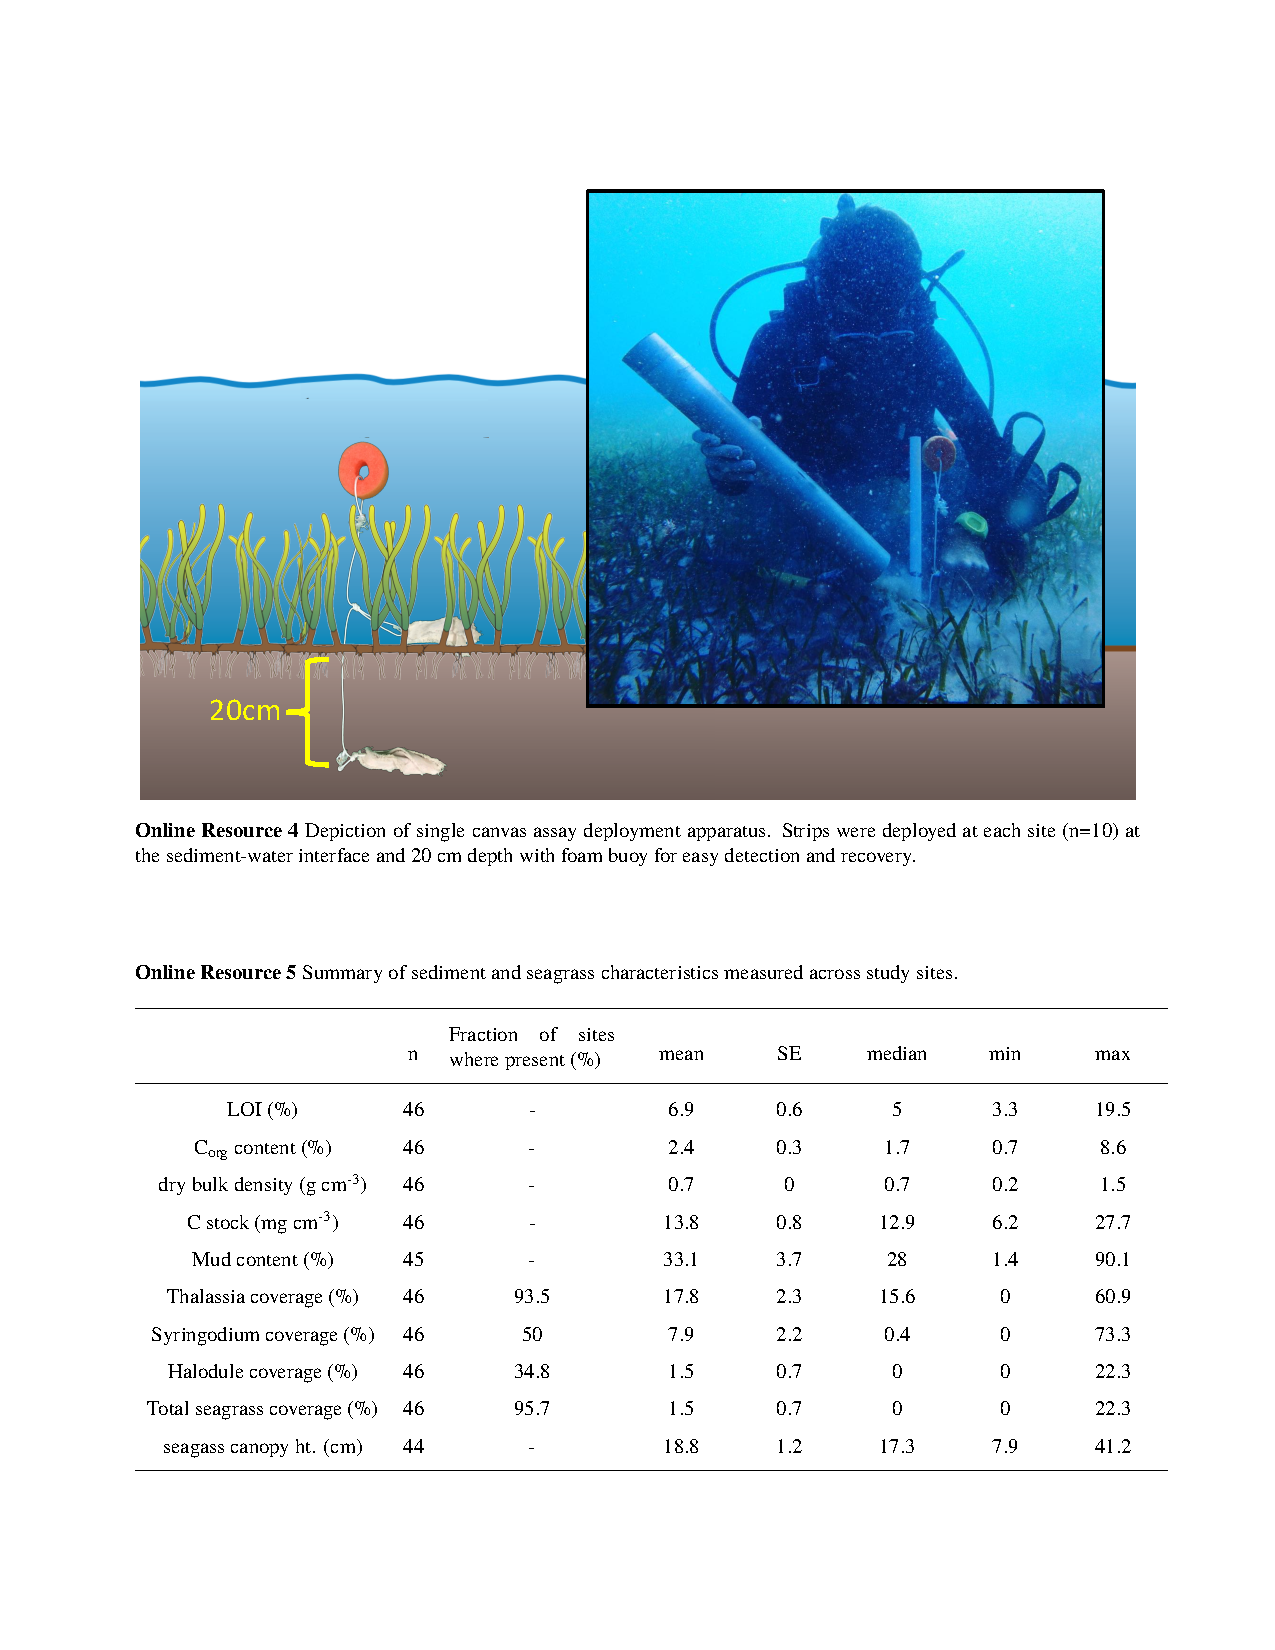
\includegraphics[width=.99\textwidth,clip, trim={1.7cm 14.2cm 1.8cm 2.6cm}]{Figures/chapter2/T3}
\caption[Summary of sediment and seagrass characteristics.]{Summary of sediment and seagrass characteristics measured at sampled south Florida sites.}
  \label{table:2T3}
\end{table}

\begin{figure}[t]
  \centering
  \includegraphics[width=.95\textwidth]{Figures/chapter2/F2}
\caption[Sediment characteristics for study sites as a function of water column depth]{Sediment characteristics for study sites as a function of water column depth}
  \label{fig:2F2}
\end{figure}

\begin{figure}[t]
  \centering
  \includegraphics[width=.95\textwidth]{Figures/chapter2/F3}
\caption[Map of sediment characteristics]{Map showing a) surface soil C\textsubscript{org} stocks, and b) sediment type across 45 study sites of Florida Bay and the Florida Keys.}
  \label{fig:2F3}
\end{figure}

\begin{figure}[t]
  \centering
  \includegraphics[width=.95\textwidth]{Figures/chapter2/F4}
\caption[Relationships between seagrasses and sediment characteristics]{Relationships between seagrasses and sediment characteristics. Each data point represents averages across ten quadrats per site and four sampling periods from January 2015 and July 2016.}
  \label{fig:2F4}
\end{figure}

\begin{figure}[t]
  \centering
  \includegraphics[width=.62\textwidth]{Figures/chapter2/F5}
\caption[Relationship between sediment type and sediment characteristics]{Relationship between sediment type and sediment characteristics. Sediment type represents averages across ten quadrats per site and four sampling periods from January 2015 and July 2016. Letters represent groupings from Tukey post-hoc tests. Gravel had only one replicate thus was excluded from significance tests.}
  \label{fig:2F5}
\end{figure}

\begin{figure}[t]
  \centering
  \includegraphics[width=.99\textwidth]{Figures/chapter2/F6}
\caption[Correlation between canvas strip tensile strength and weight loss]{Correlation between tensile strength and weight loss of canvas strips incubated in H\textsubscript{2}O\textsubscript{2} for bench top calibration experiment.}
  \label{fig:2F6}
\end{figure}

\begin{figure}[t]
  \centering
  \includegraphics[width=.95\textwidth]{Figures/chapter2/F7}
\caption[Breakdown rates for surface and buried canvas strips]{Comparison of breakdown rates for canvas strip assays deployed at 20 cm depth (\textit{buried}) and at the sediment-water interface (\textit{surface}).}
  \label{fig:2F7}
\end{figure}

\begin{figure}[t]
  \centering
  \includegraphics[width=.95\textwidth]{Figures/chapter2/F8}
\caption[Breakdown rates for canvas strip assays across grain size categories.]{Comparison of breakdown rates for canvas strip assays deployed at 20 cm depth (\textit{buried}) and at the sediment-water interface (\textit{surface}) for sites with increasingly large sediment grain size categories.}
  \label{fig:2F8}
\end{figure}
